\documentclass{article}
\usepackage{geometry}
\geometry{a4paper, landscape, margin=1.5cm}
\usepackage{graphicx}
\usepackage{caption}
\usepackage{subcaption}
\graphicspath{ {images/} }
\usepackage{listings}
\usepackage{xcolor}

\definecolor{codegreen}{rgb}{0,0.6,0}
\definecolor{codegray}{rgb}{0.5,0.5,0.5}
\definecolor{codepurple}{rgb}{0.58,0,0.82}
\definecolor{backcolour}{rgb}{1,1,1}

\lstdefinestyle{mystyle}{
    backgroundcolor=\color{backcolour},   
    commentstyle=\color{codegreen},
    keywordstyle=\color{magenta},
    numberstyle=\tiny\color{codegray},
    stringstyle=\color{codepurple},
    basicstyle=\ttfamily\footnotesize,
    breakatwhitespace=false,         
    breaklines=true,                 
    captionpos=b,                    
    keepspaces=true,                 
    numbers=left,                    
    numbersep=5pt,                  
    showspaces=false,                
    showstringspaces=false,
    showtabs=false,                  
    tabsize=2
}

\lstset{style=mystyle}

\author{\Large submitted by\\ Arghya Bandyopadhyay\\
    	RollNo. 20CS4103\\}
\title{\begin{center}
       \bfseries\Large
    	Assignment 2\\
    	Of\\
    	Network \& Distributed System Lab (CS2051)\\
        Masters of Technology in Computer Science And Engineering\\
    	\vskip1cm
    	submitted to\\
    	Dr Sujoy Saha\\
    	Assistant Professor\\
    	\&\\
    	Dr Suvrojit Das\\
    	Associate Professor\\
    	Dept. of CSE\\
    	\vskip1cm
    	
\includegraphics[width=4cm]{NITDGP}\\
    	National Institute of Technology, Durgapur\\
    \end{center}}
\date{19 June 2021}
\begin{document}
\maketitle
\pagebreak

Write TCP Chat Program.
\begin{flushleft}
\textbf{Answer.}
\end{flushleft}

\lstinputlisting[language=C]{CCode/tcpserver.c}
\pagebreak
\lstinputlisting[language=C]{CCode/tcpclient.c}
\pagebreak

\begin{figure}[h]
\begin{subfigure}{.5\textwidth}
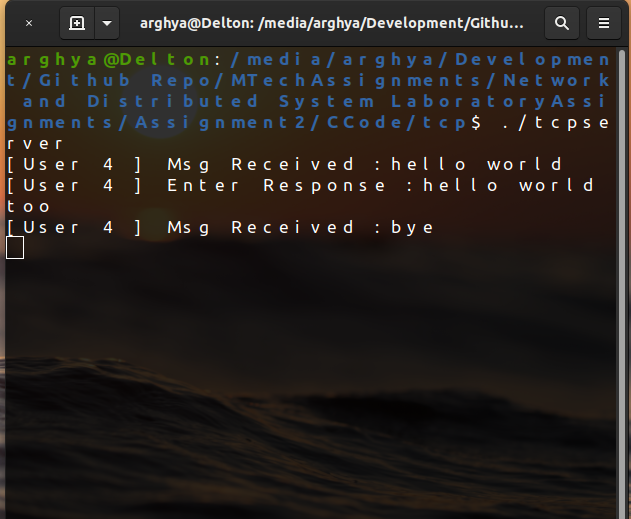
\includegraphics[width=350pt]{Output2}
\caption{TCPServer}
\label{TCPServer}
\end{subfigure}
\begin{subfigure}{.5\textwidth}
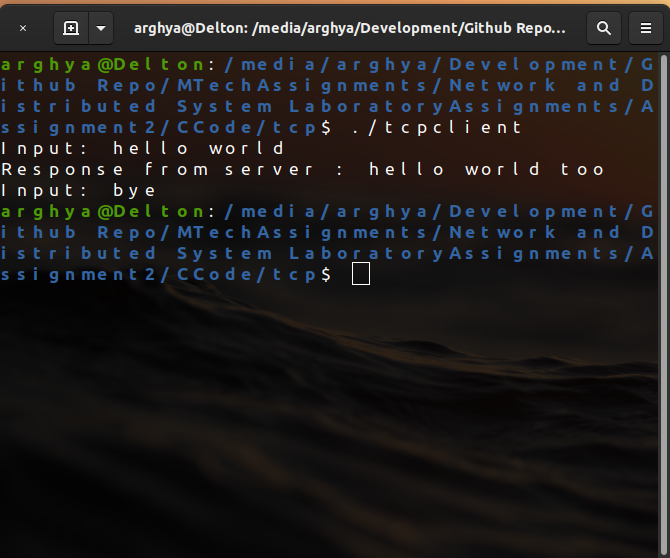
\includegraphics[width=350pt]{Output1}
\caption{TCPClient}
\label{TCPClient}
\end{subfigure}
\caption{Output:TCP}
\label{fig:TCP}
\end{figure}

\end{document}
